\chapter{Resultados Prévios}
\label{cap:resultados}

% Seleção de Projetos.
\section{Seleção de projetos}

% Critérios de seleção de repositórios.
Os critérios para a seleção de repositórios foram determinados pelos seguintes fatores:

\begin{itemize}
    \item \textbf{Ser um repositório Java:} Essencial para viabilizar a aplicação das métricas \gls{ck}.
    \item \textbf{Ser de código aberto (\textit{open-source}):} A escolha por repositórios abertos, hospedados em plataformas como o \textit{Github}, visa garantir a transparência e acessibilidade do código-fonte.
    \item \textbf{Ser ativamente mantido e atualizado:} A ativa manutenção é crucial para garantir que os repositórios estejam alinhados com as práticas e avanços mais recentes.
    \item \textbf{Ser utilizado em aplicações do mundo real:} A seleção de repositórios empregados em contextos práticos proporciona uma análise mais relevante e aplicável às situações reais.
\end{itemize}

Dessa forma, os repositórios escolhidos foram o \textit{``Apache Kafka''} \cite{KafkaGitHub} e o \textit{``ZooKeeper''} \cite{ZookeeperGitHub}. Essa escolha baseou-se no fato de os repositórios serem projetos \textit{open-source} disponíveis na plataforma GitHub, onde ambos são mantidos e atualizados de forma ativa para serem utilizados em ambientes do mundo real. Além disso, esses projetos lidam com questões altamente relevantes em \gls{sds}.

O \textit{``ZooKeeper''} desempenha um papel fundamental na coordenação e gerenciamento de serviços distribuídos. Ele oferece um serviço de consenso altamente confiável para \gls{sds}, garantindo a consistência e a sincronização entre os nós. Essa funcionalidade é crucial para a implementação de serviços distribuídos confiáveis e escaláveis, tornando o \textit{``ZooKeeper''} uma escolha valiosa para este estudo.

Por outro lado, o \textit{``Apache Kafka''} destaca-se no processamento de fluxos de dados distribuídos em larga escala. Ele fornece uma plataforma robusta para a transmissão eficiente de eventos entre diferentes componentes de um \gls{sd}. A capacidade do \textit{``Apache Kafka''} lidar com volumes massivos de dados em tempo real o torna uma solução amplamente adotada em ambientes que demandam alto desempenho e escalabilidade.

Logo, ambos os repositórios têm muito a agregar em termos de implementação e evolução, tanto para a área de \gls{sds} quanto para a \gls{es}. Assim, a escolha desses repositórios permite a análise da evolução do código em contextos práticos e desafiadores, contribuindo para uma compreensão mais abrangente das práticas de desenvolvimento em \gls{sds}.

% Métricas selecionadas inicialmente.
\section{Métricas Preliminarmente Selecionadas}

No estágio inicial desta pesquisa, optou-se por selecionar um conjunto específico de métricas, incluindo \gls{cbo}, \gls{cbom}, \gls{rfc} e \gls{wmc}. Essa escolha foi motivada pela intenção de obter uma combinação abrangente que abordasse diferentes aspectos da qualidade do código. As métricas \gls{cbo} e \gls{cbom} foram escolhidas para fornecer \textit{insights} sobre o nível de acoplamento em classes ou métodos, enquanto \gls{rfc} foi selecionada para medir o grau de comunicação entre os elementos do código. Por fim, a métrica \gls{wmc} foi incluída para avaliar a complexidade dos métodos em uma classe.

Contudo, durante o desenvolvimento do estudo, decidiu-se remover a métrica \gls{cbom} da análise. Essa decisão foi tomada devido à percepção de que a inclusão de \gls{cbom} poderia introduzir poluição nos dados, aumentando a complexidade artificialmente. Isso ocorre, por exemplo, quando a adição de uma chamada a um método da própria classe afeta negativamente a métrica. Dessa forma, a exclusão de \gls{cbom} visou manter a integridade e a precisão das métricas escolhidas, proporcionando uma análise mais clara e objetiva da evolução do código.

% Desenvolvimento das ferramentas disponíveis no GitHub feitas em Python.
\section{Desenvolvimento da ferramenta}

As ferramentas desenvolvidas podem ser encontradas no Github \footnote{https://github.com/BrenoFariasdaSilva/Scientific-Research}, estando as três primeiras no diretório ``\textit{PyDriller}'' e as duas últimas no diretório ``\textit{RefactoringMiner}'', sendo que todas foram feitas usando a linguagem de programação Python \cite{PythonProgrammingLanguage}.

A primeira ferramenta desenvolvida, denominada \textit{code\_metrics.py} \cite{PyDriller:CodeMetrics:2023}, está integrada ao \textit{PyDriller} e ao \gls{ck}. Durante esse processo, a ferramenta percorre toda a árvore de \textit{commits} de um repositório específico. Para cada \textit{commit}, o \gls{ck} é executado, resultando na geração das métricas \gls{ck} para cada estado do repositório ao final da execução. Adicionalmente, a ferramenta produz um \textit{diff} para cada refatoração realizada no repositório, possibilitando a investigação das refatorações realizadas no código em caso de identificação de uma tendência de melhoria das métricas.

A segunda ferramenta desenvolvida, denominada \textit{metrics\_changes.py} \cite{PyDriller:MetricsChanges:2023},  depende da execução da primeira para operar. Essencialmente, esta ferramenta percorre as métricas de todos os estados do repositório processado, produzindo os seguintes resultados:

\begin{itemize}
    \item \textbf{Evolução das métricas}: Geração de arquivos divididos por classe e métodos, contendo o histórico completo de alterações em cada classe ou método, incluindo suas métricas correspondentes.
    \item \textbf{Predição das métricas}: Criação de arquivos segmentados por classe e métodos, apresentando uma predição baseada na regressão linear aplicada às métricas analisadas, utilizando o histórico gerado anteriormente.
    \item \textbf{Estatísticas das métricas}: Produção de um arquivo para classes e outro para métodos, ordenados pelo número de alterações efetuadas em cada classe ou método.
    \item \textbf{Alterações substanciais nas métricas}: Identificação de padrões de decréscimo do \gls{cbo}, oferecendo uma análise detalhada das classes ou métodos que apresentam tendências de melhoria ao longo do tempo.
\end{itemize}

Assim, resumidamente, esse projeto gera metadados que facilitam a análise dos códigos, reduzindo o escopo de busca por refatorações que, à luz das métricas, são consideradas relevantes para nosso estudo. Vale ressaltar que, enquanto o estudo que desenvolve o \textit{DistFax} \cite{DistFax} utiliza métricas \gls{ipc} dinâmicas (geradas em tempo de execução), o presente estudo emprega métricas de código estáticas (geradas apenas pela análise do código-fonte). Isso se deve à inadequação das métricas tradicionais para medir a qualidade das trocas de mensagens em \gls{sds}, pois eles não se baseiam em relações explícitas, analisam apenas um computador e não consideram o sistema em sua totalidade. Embora o uso dessas métricas pudesse ser benéfico, o custo computacional pode ser bastante significativo para calcular todas elas.
As figuras a seguir apresentam exemplos das saídas geradas por esse algoritmo:

\begin{figure}[h]
    \centering
    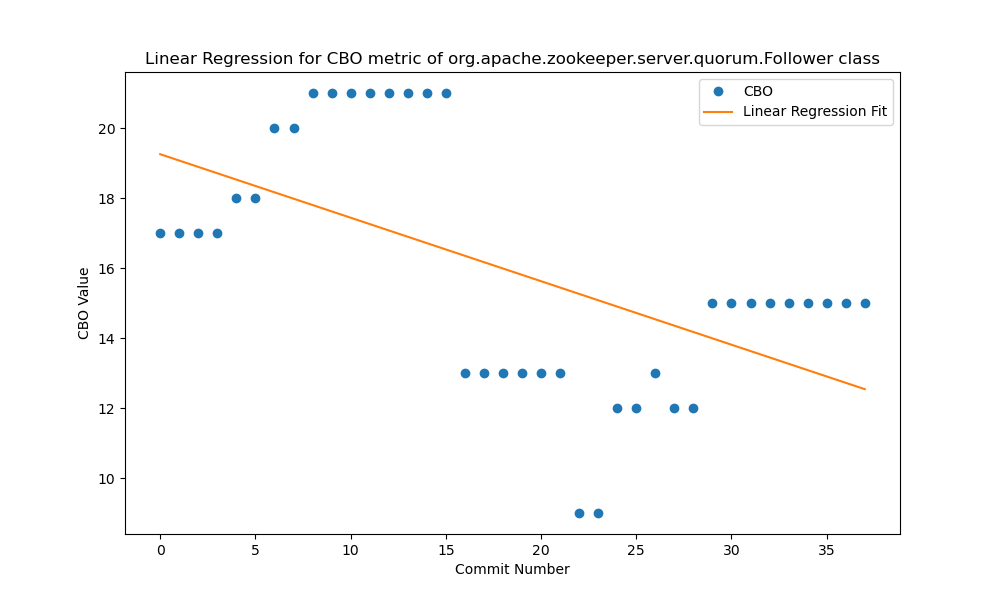
\includegraphics[width=0.8\linewidth]{figuras/Output/Metrics_Predictions/CBO.png}
    \caption{Regressão linear da métrica \gls{cbo} da classe org.apache.zookeeper.server.quorum.Follower}
    \label{fig:RlCBO}
\end{figure}

\begin{figure}[h]
    \centering
    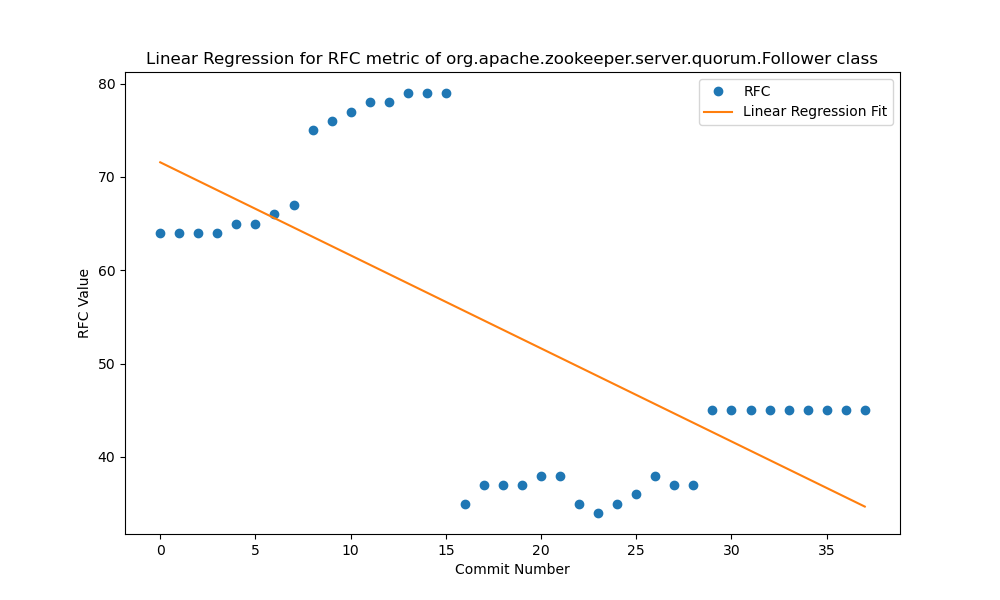
\includegraphics[width=0.8\linewidth]{figuras/Output/Metrics_Predictions/RFC.png}
    \caption{Regressão linear da métrica \gls{rfc} da classe org.apache.zookeeper.server.quorum.Follower}
    \label{fig:RlRFC}
\end{figure}

\begin{figure}[h]
    \centering
    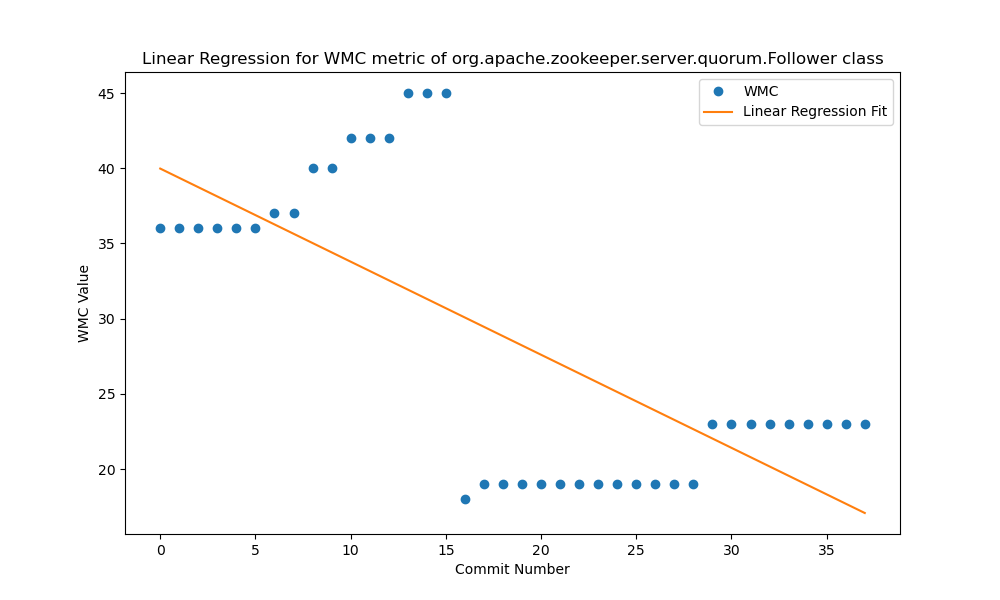
\includegraphics[width=0.8\linewidth]{figuras/Output/Metrics_Predictions/WMC.png}
    \caption{Regressão linear da métrica \gls{wmc} da classe org.apache.zookeeper.server.quorum.Follower}
    \label{fig:RlWMC}
\end{figure}

\begin{figure}[h]
    \centering
    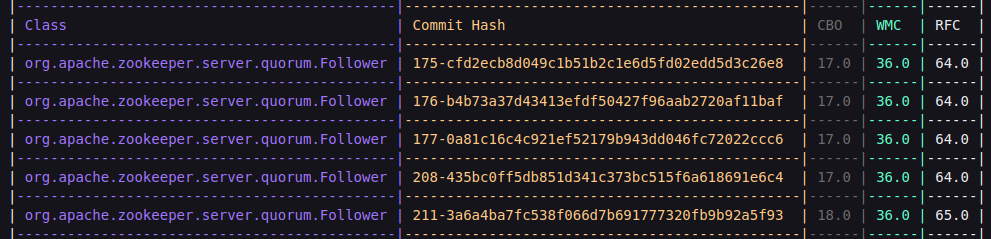
\includegraphics[width=0.8\linewidth]{figuras/Output/Metrics_Evolution/Metrics_Evolution.png}
    \caption{Evolução das métricas da classe org.apache.zookeeper.server.quorum.Follower}
    \label{fig:EvolutionFollowerClass}
\end{figure}

\begin{figure}[h]
    \centering
    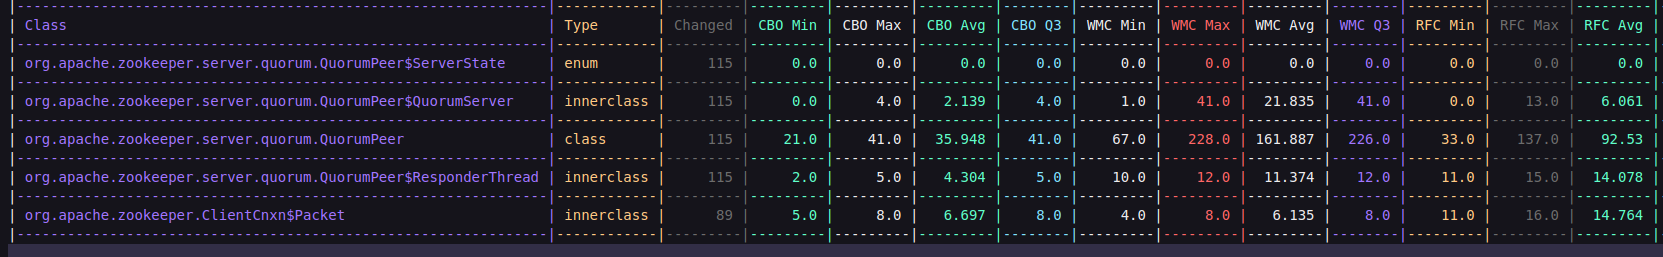
\includegraphics[width=0.8\linewidth]{figuras/Output/Metrics_Statistics/Metrics_Statistics.png}
    \caption{Estatísticas das métricas do ZooKeeper}
    \label{fig:StatisticsFollowerClass}
\end{figure}

As Figuras \ref{fig:RlCBO}, \ref{fig:RlRFC} e \ref{fig:RlWMC} proporcionam uma perspectiva visual das tendências nas métricas \gls{cbo}, \gls{rfc} e \gls{wmc} específicas da classe \textit{org.apache.zookeeper.server.quorum.Follower}. Enquanto isso, as figuras \ref{fig:EvolutionFollowerClass} e \ref{fig:StatisticsFollowerClass} apresentam um vislumbre das cinco primeiras linhas dos \textit{CSVs} gerados, delineando a evolução das métricas de tal classe e as estatísticas gerais das classes no contexto do \textit{ZooKeeper}. As primeiras três imagens oferecem uma compreensão aprofundada do comportamento evolutivo dessa classe específica, enquanto a última concentra-se nas classes mais frequentemente modificadas, destacando sua propensão a refatorações significativas ou sua relevância fundamental dentro do ecossistema do \textit{ZooKeeper}.

A \href{https://github.com/BrenoFariasdaSilva/Scientific-Research/blob/main/PyDriller/Scripts/track_files.py}{terceira ferramenta} desenvolvida, mais uma vez, depende da execução da primeira para funcionar. Em suma, esta ferramenta busca por arquivos específicos nos \textit{diffs} dos repositórios. Neste estudo, ela foi utilizada para localizar arquivos de comentários sobre as refatorações realizadas em um \textit{commit}, como o arquivo ``CHANGES.txt'', uma vez que o espaço da mensagem do \textit{commit} pode oferecer uma visão limitada das refatorações efetuadas.

A \href{https://github.com/BrenoFariasdaSilva/Scientific-Research/blob/main/PyDriller/Scripts/track_files.py}{quarta} e a \href{https://github.com/BrenoFariasdaSilva/Scientific-Research/blob/main/RefactoringMiner/metrics_evolution_refactors.py}{quinta ferramenta} desenvolvidas são substancialmente similares, distinguindo-se apenas no escopo de aplicação, onde a quarta  incide sobre a totalidade do repositório, enquanto a quinta é específica para classes ou métodos dentro do repositório. Ambas as ferramentas compartilham um funcionamento comum, fazendo uso da ferramenta Refactoring Miner \cite{Tsantalis:ICSE:2018:RefactoringMiner}.

O processo inicia-se com a utilização da ferramenta \textit{RefactoringMiner}, a qual, por meio da extração do histórico de \textit{commits}, analisa os \textit{diffs}, identificando padrões de refatorações. O \textit{RefactoringMiner} possui um banco de dados de refatorações previamente detectadas, permitindo uma análise eficiente das mudanças no código-fonte. A ferramenta gera uma saída estruturada que lista as refatorações identificadas, indicando quais arquivos e linhas de código foram afetados em cada \textit{commit}.

Essa saída estruturada proporciona uma base sólida para análises mais aprofundadas, permitindo uma compreensão detalhada das refatorações realizadas ao longo do tempo. A capacidade de distinguir entre o repositório inteiro (quarta ferramenta) e componentes específicos, como classes ou métodos (quinta ferramenta), amplia a flexibilidade dessas ferramentas, adaptando-as às necessidades específicas de investigação e análise de refatorações em projetos de software.

A saída dos algoritmos que utilizam o \textit{RefactoringMiner} consiste em um objeto \textit{JSON}, semelhante à Figura \ref{fig:RefactoringMinerOutput}, que permite a análise das refatorações por tipo. Destaca-se que, a partir do \textit{JSON} geral, é possível aplicar filtros para armazenar apenas refatorações dos tipos desejados. Essa abordagem proporciona uma visão detalhada e personalizável das transformações efetuadas no código-fonte.

\begin{figure}[h]
    \centering
    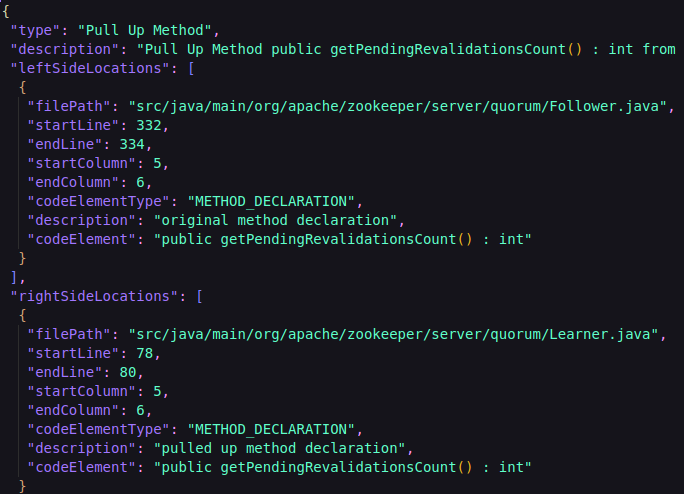
\includegraphics[width=0.8\linewidth]{figuras/Output/RefactoringMiner/org.apache.zookeeper.server.quorum.Learner.png}
    \caption{Refatorações da classe org.apache.zookeeper.server.quorum.Learner}
    \label{fig:RefactoringMinerOutput}
\end{figure}

% Análise das métricas dos projetos selecionados.
\section{Análise das métricas dos projetos selecionados}
Apesar da intenção inicial de analisar dois repositórios, o \textit{``Apache Kafka''} e o \textit{``ZooKeeper''}, até o momento, concentramos nossos esforços exclusivamente no exame do repositório do \textit{``ZooKeeper''}. Esta escolha se fundamenta no tamanho inferior deste repositório em comparação com o \textit{``Apache Kafka''}, permitindo uma análise mais focalizada e a possibilidade de apresentar resultados preliminares neste trabalho. A decisão foi motivada por considerações de limitação de tempo, pois a análise detalhada de um único repositório já representa um desafio significativo, demandando uma abordagem minuciosa para compreender a evolução do código-fonte e as refatorações realizadas.  Neste trabalho, serão mencionados alguns casos analisados que aparentavam ser promissores, no entanto, mostraram algumas dificuldades a mais que iremos lidar nos estágios seguintes deste projeto de pesquisa.

A análise atual revela a presença de vários \textit{commits} no histórico do repositório do \textit{``ZooKeeper''}, e notou-se uma tendência decrescente no valor de métricas, como o \gls{cbo}. No entanto, é crucial observar que apenas uma parcela restrita desses \textit{commits} inclui mensagens associadas a melhorias de desempenho, segurança, substituição de algoritmos ou melhorias de modo geral. 

Lamentavelmente, até o momento, apenas um \textit{commit} apresentou uma correlação direta entre as vulnerabilidades identificadas no banco de dados do \textit{``CVE-Details''} e os \textit{commits} no repositório do \textit{ZooKeeper}. O único caso encontrado foi para o \textit{commit} 9213f7353b1e6ce4d0fdbc1dca963ace1fd32cec, o qual relaciona-se a vulnerabilidade CVE-2021-21295. Entretando, por mais que o \textit{commit} resolva um problema de vulnerabilidade, constatamos que esta refatoração específica consiste apenas na atualização da versão da biblioteca \textit{Netty} no arquivo pom.xml do Java, o qual prove uma estrutura cliente-servidor de E/S não bloqueante, logo ela não se mostra uma boa candidata para correlacionar métricas de código com a segurança, pois se trata de uma ação direta para resolver uma vulnerabilidade conhecida.

A análise do \textit{commit} 83cf0a93c37759334fab885c2010fa0b7d953f52 foi aprofundada, cuja mensagem é ``\textit{ZOOKEEPER-308. Improve the atomic broadcast performance in 3x}''. Apesar da indicação inicial de um ganho de desempenho em 3 vezes, uma investigação mais detalhada revelou que a alteração se limitava à substituição da classe \textit{FileOutputStream''} por \textit{BufferedOutputStream''}. Embora essa mudança resulte em melhoria de desempenho, não constitui uma refatoração significativa, pois o \textit{commit} altera 19 arquivos, sendo relevante apenas o arquivo ``\textit{FileTxnLog.java}'', que consiste na troca das classes mencionadas. Os outros arquivos alterados abordam refatorações relacionadas à validação de objetos nulos antes de operações, mas estão fora do escopo da mensagem do \textit{commit}. Apesar disso, a melhoria de desempenho é reconhecida como válida, embora sua magnitude não possa ser verificada.

Embora a mudança promova efetivamente uma melhoria de desempenho, as métricas tradicionais de código, como \gls{cbo}, \gls{rfc} e \gls{wmc}, podem não refletir diretamente essa otimização. Tais métricas podem não capturar aspectos específicos relacionados à eficiência de operações de entrada e saída. Portanto, apesar da magnitude do aprimoramento não poder ser totalmente verificada por meio das métricas convencionais, é valida a melhoria de desempenho proporcionada pela otimização do uso da classe de E/S, mas não relevante para a criação de um exemplo trabalhado. Em síntese, as métricas tradicionais não capturam completamente a magnitude do ganho de desempenho. No entanto, é reconhecida a validade da otimização introduzida pelo \textit{commit}, ressaltando a importância de uma análise contextualizada para compreender a relação entre alterações de código, mensagens de \textit{commit} e métricas de código.

\begin{figure}[h]
    \centering
    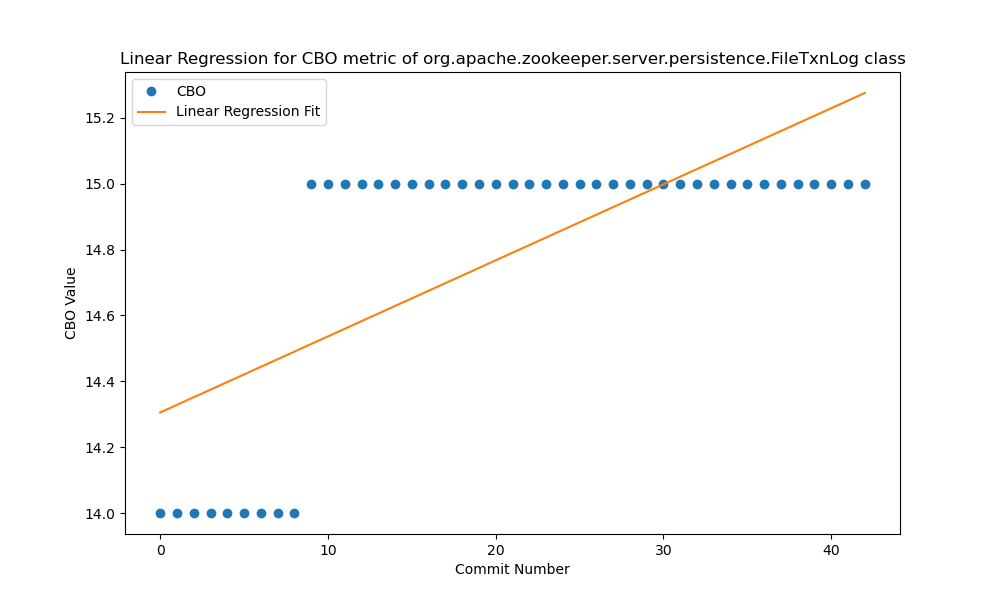
\includegraphics[width=0.8\linewidth]{figuras/343-83cf0a93c37759334fab885c2010fa0b7d953f52/Class-org.apache.zookeeper.server.persistence.FileTxnLog/CBO.png}
    \caption{CBO da classe \textit{org.apache.zookeeper.server.persistence.FileTxnLog}.}
    \label{fig:CBO3xPerformanceClass}
\end{figure}

\begin{figure}[h]
    \centering
    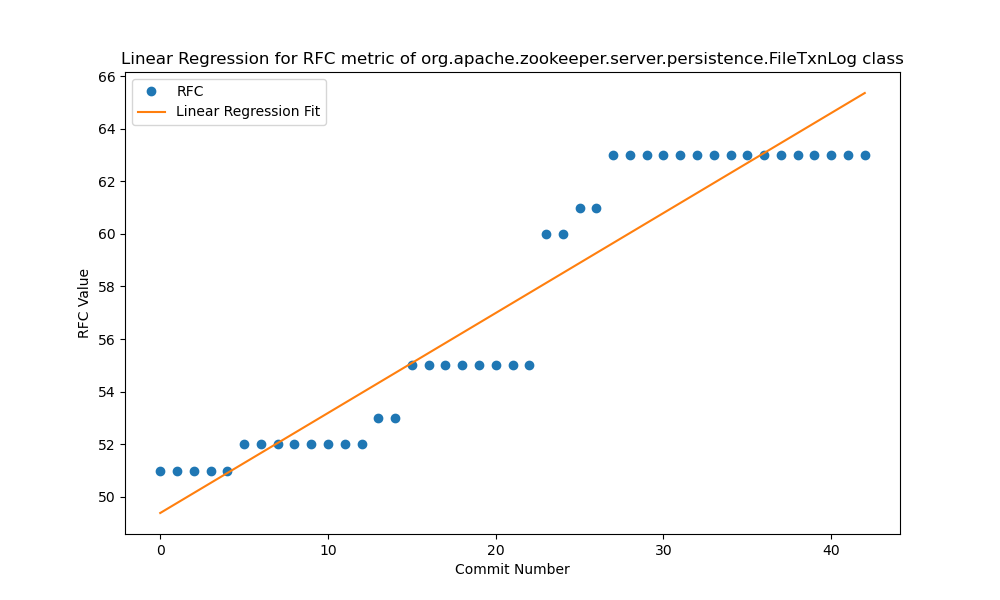
\includegraphics[width=0.8\linewidth]{figuras/343-83cf0a93c37759334fab885c2010fa0b7d953f52/Class-org.apache.zookeeper.server.persistence.FileTxnLog/RFC.png}
    \caption{RFC da classe \textit{org.apache.zookeeper.server.persistence.FileTxnLog}.}
    \label{fig:RFC3xPerformanceClass}
\end{figure}

\begin{figure}[h]
    \centering
    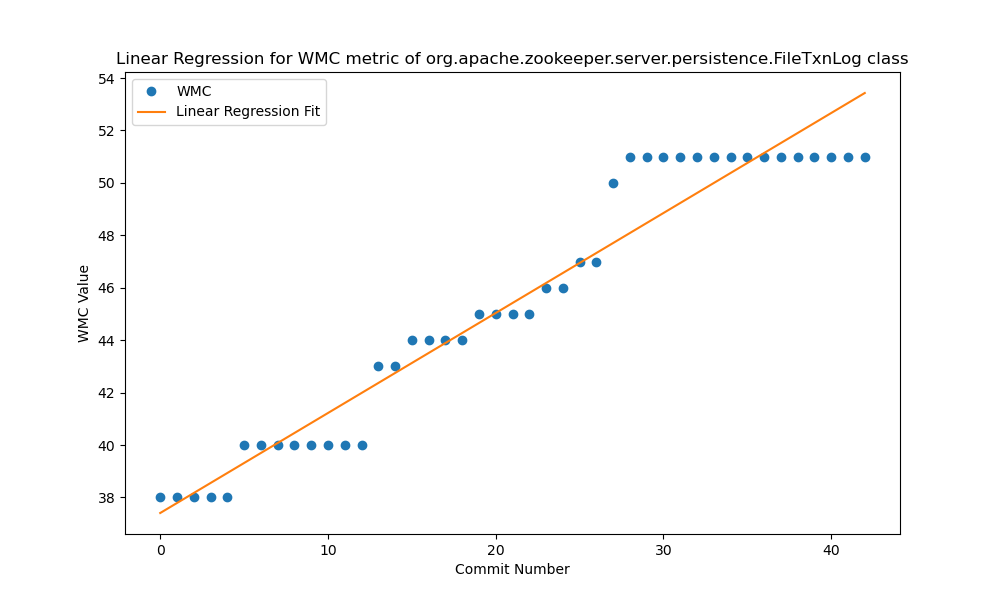
\includegraphics[width=0.8\linewidth]{figuras/343-83cf0a93c37759334fab885c2010fa0b7d953f52/Class-org.apache.zookeeper.server.persistence.FileTxnLog/WMC.png}
    \caption{WMC da classe \textit{org.apache.zookeeper.server.persistence.FileTxnLog}.}
    \label{fig:WMC3xPerformanceClass}
\end{figure}

A falta de uma refatoração mais substancial e a existência de uma melhoria de desempenho que não pôde ser validada tornam este \textit{commit} inadequado para servir como objeto de exemplo trabalhado. Além disso, uma vez que a classe \textit{``BufferedOutputStream''} está presente desde a versão inicial do Java (lançada em 1996) e o \textit{commit} em questão é de 2009, ou seja, o uso de um \textit{buffered input} devia ter sido feita desde o começo do projeto.

% Adicionar pelo menos mais um exemplo de commit analisado.

Observou-se que parte da complexidade na análise de um \textit{commit} propriamente dito reside na existência de uma considerável poluição nos dados. Muitos \textit{commits} no repositório do \textit{``ZooKeeper''} abrangem alterações em inúmeros arquivos, frequentemente incorporando refatorações não diretamente correlacionadas às mensagens de \textit{commit}. Essa complexidade aumenta a dificuldade de discernir as motivações subjacentes por trás das mudanças no código-fonte, tornando desafiador o processo de vincular essas alterações a possíveis vulnerabilidades identificadas externamente. Este fenômeno destaca a importância de uma abordagem criteriosa na interpretação do histórico de \textit{commits} para extrair conclusões significativas sobre a evolução do \textit{software} em relação à qualquer aspecto desejado.

\section{Limitações}
\label{sec:limitacoes}

% Limitações do projeto de pesquisa.
Este trabalho apresenta uma limitação, a qual reside na impossibilidade de realizar análises empíricas de certas melhorias de desempenho, como a análise das trocas de mensagens em tempo real, devido à restrição ao uso de métricas estáticas de código. Isso impede a avaliação prática por meio da execução de \gls{sds} e simulações em grande escala, representando uma restrição na obtenção de percepções detalhadas sobre o desempenho em contextos de uma quantidade massiva de requisições sendo enviadas ao \gls{sd}. Além disso, poucos repositórios usam a conveção de \textit{commits}, o que facilitaria obter refatorações significativas, não poluídas por refatorações irrelevantes \cite{conventionalcommits}.